% -*- TeX-engine: xetex; -*-
% Compile with XeLaTeX

%%%%%%%%%%%%%%%%%%%%%%%
% To do before class
%%%%%%%%%%%%%%%%%%%%%%%

% Send the Logistics/Week0Annoucnement (the night before).
% Send an email reminding students to bring a charged computer (the night before).

%%%%%%%%%%%%%%%%%%%%%%%
% Option 1: Slides: (comment for handouts)   %
%%%%%%%%%%%%%%%%%%%%%%%

\documentclass[slidestop,compress,mathserif,12pt,t,professionalfonts,xcolor=table]{beamer}

% solution stuff
\newcommand{\solnMult}[1]{
\only<1>{#1}
\only<2->{\red{\textbf{#1}}}
}
\newcommand{\soln}[1]{\textit{#1}}

%%%%%%%%%%%%%%%%%%%%%%%%%%%%%%%
% Option 2: Handouts, without solutions (post before class)    %
%%%%%%%%%%%%%%%%%%%%%%%%%%%%%%%

% \documentclass[11pt,containsverbatim,handout,xcolor=xelatex,dvipsnames,table]{beamer}

% % handout layout
% \usepackage{pgfpages}
% \pgfpagesuselayout{4 on 1}[letterpaper,landscape,border shrink=5mm]

% % solution stuff
% \newcommand{\solnMult}[1]{#1}
% \newcommand{\soln}[1]{}

% % % This breaks things for me for some reason.
% % tell pgfpages how to set page sizes in XeLaTeX
% %\renewcommand\pgfsetupphysicalpagesizes{%
% %   \pdfpagewidth\pgfphysicalwidth\pdfpageheight\pgfphysicalheight%
% %}

%%%%%%%%%%%%%%%%%%%%%%%%%%%%%%%%%%%%
% Option 3: Handouts, with solutions (may post after class if need be)    %
%%%%%%%%%%%%%%%%%%%%%%%%%%%%%%%%%%%%

% \documentclass[11pt,containsverbatim,handout,xcolor=xelatex,dvipsnames,table]{beamer}

% % handout layout
% \usepackage{pgfpages}
% \pgfpagesuselayout{4 on 1}[letterpaper,landscape,border shrink=5mm]

% % solution stuff
% \newcommand{\solnMult}[1]{\red{\textbf{#1}}}
% \newcommand{\soln}[1]{\textit{#1}}

% % % This breaks things for me for some reason.
% % % tell pgfpages how to set page sizes in XeLaTeX
% % \renewcommand\pgfsetupphysicalpagesizes{%
% %    \pdfpagewidth\pgfphysicalwidth\pdfpageheight\pgfphysicalheight%
% % }

%%%%%%%%%%%%%%%%%%%%%%%%%%%%%%%
% Option 4: Notes Only
%%%%%%%%%%%%%%%%%%%%%%%%%%%%%%%

% % See http://tex.stackexchange.com/questions/114219/add-notes-to-latex-beamer
% \documentclass[10pt,containsverbatim,xcolor=xelatex,dvipsnames,table,notes=only]{beamer}

% % handout layout
% % \usepackage{pgfpages}
% % \pgfpagesuselayout{1 on 1}[letterpaper, landscape, border shrink=5mm]

% % solution stuff
% \newcommand{\solnMult}[1]{#1}
% \newcommand{\soln}[1]{}

% % % Having a problem with this.
% % tell pgfpages how to set page sizes in XeLaTeX
% % \renewcommand\pgfsetupphysicalpagesizes{%
% %   \pdfpagewidth\pgfphysicalwidth\pdfpageheight\pgfphysicalheight%
% %}

%%%%%%%%%%
% Load style file, defaults  %
%%%%%%%%%%

%%%%%%%%%%%%%%%%
% Themes
%%%%%%%%%%%%%%%%

% See http://deic.uab.es/~iblanes/beamer_gallery/ for mor options

% Style theme
\usetheme{Pittsburgh}

% Color theme
\usecolortheme{seahorse}

% Font theme
%\usepackage[T1]{fontenc}
%\usepackage[scaled=0.92]{helvet}

%\usepackage[no-math]{fontspec}
%\setsansfont{TeX Gyre Heros}
% "TeX Gyre Heros can be used as a replacement for Helvetica"
% In Unix, unzip the following into ~/.fonts
% In Mac, unzip it, double-click the .otf files, and install using "FontBook"
%   http://www.gust.org.pl/projects/e-foundry/tex-gyre/heros/qhv2.004otf.zip

\usepackage{fontspec}

%%%%%%%%%%%%%%%%
% Packages
%%%%%%%%%%%%%%%%

\usepackage{geometry}
\usepackage{graphicx}
\usepackage{amssymb}
\usepackage{epstopdf}
\usepackage{amsmath}  	% this permits text in eqnarray among other benefits
\usepackage{url}		% produces hyperlinks
\usepackage[english]{babel}
\usepackage[latin1]{inputenc}
\usepackage{colortbl}	% allows for color usage in tables
\usepackage{multirow}	% allows for rows that span multiple rows in tables
\usepackage{color}		% this package has a variety of color options
\usepackage{colortbl}
\usepackage{pgf}
\usepackage{calc}
\usepackage{ulem}
\usepackage{multicol}
\usepackage{textcomp}
\usepackage{txfonts}
\usepackage{listings}
\usepackage{tikz}
\usepackage{fancyvrb}

%%%%%%%%%%%%%%%%
% Remove navigation symbols
%%%%%%%%%%%%%%%%

\beamertemplatenavigationsymbolsempty
\hypersetup{pdfpagemode=UseNone} % don't show bookmarks on initial view

%%%%%%%%%%%%%%%%
% User defined colors
%%%%%%%%%%%%%%%%

% Pantone 2015 Spring colors
% http://iwork3.us/2014/09/16/pantone-2015-spring-fashion-report/
% update each semester or year

\xdefinecolor{custom_blue}{rgb}{0, 0.70, 0.79} % scuba blue
\xdefinecolor{custom_darkBlue}{rgb}{0.11, 0.31, 0.54} % classic blue
\xdefinecolor{custom_orange}{rgb}{0.97, 0.57, 0.34} % tangerine
\xdefinecolor{custom_green}{rgb}{0.49, 0.81, 0.71} % lucite green
\xdefinecolor{custom_red}{rgb}{0.58, 0.32, 0.32} % marsala

\xdefinecolor{custom_lightGray}{rgb}{0.78, 0.80, 0.80} % glacier gray
\xdefinecolor{custom_darkGray}{rgb}{0.54, 0.52, 0.53} % titanium

%%%%%%%%%%%%%%%%
% Template colors
%%%%%%%%%%%%%%%%

\setbeamercolor*{palette primary}{fg=white,bg= custom_blue}
\setbeamercolor*{palette secondary}{fg=black,bg= custom_blue!80!black}
\setbeamercolor*{palette tertiary}{fg=white,bg= custom_blue!80!black!80}
\setbeamercolor*{palette quaternary}{fg=white,bg= custom_blue}

\setbeamercolor{structure}{fg= custom_blue}
\setbeamercolor{frametitle}{bg= custom_blue!90}
\setbeamertemplate{blocks}[shadow=false]
\setbeamersize{text margin left=2em,text margin right=2em}

%%%%%%%%%%%%%%%%
% Styling fonts, bullets, etc.
%%%%%%%%%%%%%%%%

% styling of itemize bullets
\setbeamercolor{item}{fg=custom_blue}
\setbeamertemplate{itemize item}{{{\small$\blacktriangleright$}}}
\setbeamercolor{subitem}{fg=custom_blue}
\setbeamertemplate{itemize subitem}{{\textendash}}
\setbeamerfont{itemize/enumerate subbody}{size=\footnotesize}
\setbeamerfont{itemize/enumerate subitem}{size=\footnotesize}

% styling of enumerate bullets
\setbeamertemplate{enumerate item}{\insertenumlabel.}
\setbeamerfont{enumerate item}{family={\fontspec{Helvetica Neue}}}
\setbeamerfont{enumerate subitem}{family={\fontspec{Helvetica Neue}}}
\setbeamerfont{enumerate subsubitem}{family={\fontspec{Helvetica Neue}}}

% make frame titles small to make room in the slide
\setbeamerfont{frametitle}{size=\small} 

% set Helvetica Neue font for frame and section titles
\setbeamerfont{frametitle}{family={\fontspec{Helvetica Neue}}}
\setbeamerfont{sectiontitle}{family={\fontspec{Helvetica Neue}}}
\setbeamerfont{section in toc}{family={\fontspec{Helvetica Neue}}}
\setbeamerfont{subsection in toc}{family={\fontspec{Helvetica Neue}}, size=\small}
\setbeamerfont{footline}{family={\fontspec{Helvetica Neue}}}
\setbeamerfont{subsection in toc}{family={\fontspec{Helvetica Neue}}}
\setbeamerfont{block title}{family={\fontspec{Helvetica Neue}}}

%%%%%%%%%%%%%%%%
% Color text commands
%%%%%%%%%%%%%%%%

%orange
\newcommand{\orange}[1]{\textit{\textcolor{custom_orange}{#1}}}

% green
\newcommand{\green}[1]{\textit{\textcolor{custom_green}{#1}}}

% red
\newcommand{\red}[1]{\textit{\textcolor{custom_red}{#1}}}

% dark gray
\newcommand{\darkgray}[1]{\textit{\textcolor{custom_darkGray}{#1}}}

% light gray
\newcommand{\lightgray}[1]{\textit{\textcolor{custom_lightGray}{#1}}}


%%%%%%%%%%%%%%%%
% Custom commands
%%%%%%%%%%%%%%%%

% cancel
\newcommand{\cancel}[1]{%
    \tikz[baseline=(tocancel.base)]{
        \node[inner sep=0pt,outer sep=0pt] (tocancel) {#1};
        \draw[red, line width=0.5mm] (tocancel.south west) -- (tocancel.north east);
    }%
}

% degree
\newcommand{\degree}{\ensuremath{^\circ}}

% cite
\newcommand{\ct}[1]{
\vfill
{\tiny #1}}

% Note
\newcommand{\Note}[1]{
\rule{2.5cm}{0.25pt} \\ \textit{\footnotesize{\textcolor{custom_red}{Note:} \textcolor{custom_darkGray}{#1}}}}

% Remember
\newcommand{\Remember}[1]{\textit{\scriptsize{\textcolor{custom_red}{Remember:} #1}}}

% links: webURL, webLink
\newcommand{\webURL}[1]{\urlstyle{same}{\textit{\textcolor{custom_blue}{\url{#1}}}}}
\newcommand{\webLink}[2]{\href{#1}{\textcolor{custom_blue}{{#2}}}}

% mail
\newcommand{\mail}[1]{\href{mailto:#1}{\textit{\textcolor{custom_blue}{#1}}}}

% highlighting: hl, hlGr, mathhl
\newcommand{\hl}[1]{\textit{\textcolor{custom_blue}{#1}}}
\newcommand{\hlGr}[1]{\textit{\textcolor{custom_green}{#1}}}
\newcommand{\mathhl}[1]{\textcolor{custom_blue}{\ensuremath{#1}}}

% example
\newcommand{\ex}[1]{\textcolor{blue}{{{\small (#1)}}}}

% two col: two columns
\newenvironment{twocol}[4]{
\begin{columns}[c]
\column{#1\textwidth}
#3
\column{#2\textwidth}
#4
\end{columns}
}

% slot (for probability calculations)
\newenvironment{slot}[2]{
\begin{array}{c} 
\underline{#1} \\ 
#2
\end{array}
}

% pr: left and right parentheses
\newcommand{\pr}[1]{
\left( #1 \right)
}

%%%%%%%%%%%%%%%%
% Custom blocks
%%%%%%%%%%%%%%%%

% activity: less commonly used
\newcommand{\activity}[2]{
\setbeamertemplate{itemize item}{{{\small\textcolor{custom_orange}{$\blacktriangleright$}}}}
\setbeamercolor{block title}{fg=white, bg=custom_orange}
\setbeamerfont{block title}{size=\small}
\setbeamercolor{block body}{fg=black, bg=custom_orange!20!white!80}
\setbeamerfont{block body}{size=\small}
\begin{block}{Activity: #1}
#2
\end{block}
}

% app: application exercise
\newcommand{\app}[2]{
\setbeamercolor{block title}{fg=white,bg=custom_green}
\setbeamercolor{block body}{fg=black,bg=custom_green!20!white!80}
\begin{block}{{\small Application exercise: #1}}
#2
\end{block}
}

% disc: discussion question
\newcommand{\disc}[1]{
\setbeamercolor{block body}{bg=custom_blue!25!white!80, fg=custom_blue!55!black!95}
\begin{block}{\vspace*{-3ex}}
#1
\end{block}
}

% clicker: clicker question
\newcommand{\clicker}[1]{
\setbeamercolor{block title}{bg=custom_blue!80!white!50,fg=custom_blue!30!black!90}
\setbeamercolor{block body}{bg=custom_blue!20!white!80,fg=custom_blue!30!black!90}
\begin{block}{\vspace*{-0.2ex}{\footnotesize Clicker question}\vspace*{-0.2ex}}
#1
\end{block}
}

% formula
\newcommand{\formula}[2]{
\setbeamercolor{block title}{bg=custom_blue!40!white!60,fg=custom_blue!55!black!95}
\begin{block}{{\small#1}}
#2
\end{block}
}

% code
\newcommand{\code}[1]{
\newfontfamily{\monaco}{Monaco}
{\monaco {\footnotesize \textcolor{custom_darkBlue}{#1}}}
}

% output
\renewcommand{\output}[1]{
{\monaco {\footnotesize \textcolor{custom_darkGray}{#1}}}
}

%%%%%%%%%%%%%%%%
% Change margin
%%%%%%%%%%%%%%%%

\newenvironment{changemargin}[2]{%
\begin{list}{}{%
\setlength{\topsep}{0pt}%
\setlength{\leftmargin}{#1}%
\setlength{\rightmargin}{#2}%
\setlength{\listparindent}{\parindent}%
\setlength{\itemindent}{\parindent}%
\setlength{\parsep}{\parskip}%
}%
\item}{\end{list}}

%%%%%%%%%%%%%%%%
% Footnote
%%%%%%%%%%%%%%%%

\long\def\symbolfootnote[#1]#2{\begingroup%
\def\thefootnote{\fnsymbol{footnote}}\footnote[#1]{#2}\endgroup}

%%%%%%%%%%%%%%%%
% Graphics
%%%%%%%%%%%%%%%%

\DeclareGraphicsRule{.tif}{png}{.png}{`convert #1 `dirname #1`/`basename #1 .tif`.png}

%%%%%%%%%%%%%%%%
% Slide number
%%%%%%%%%%%%%%%%

\setbeamertemplate{footline}{%
    \raisebox{5pt}{\makebox[\paperwidth]{\hfill\makebox[20pt]{\color{gray}
          \scriptsize\insertframenumber}}}\hspace*{5pt}}

          
%%%%%%%%%%%%%%%%
% Remove page numbers
%%%%%%%%%%%%%%%%

\newcommand{\removepagenumbers}{% 
  \setbeamertemplate{footline}{}
}

%%%%%%%%%%%%%%%%
% TOC slides
%%%%%%%%%%%%%%%%

% TRY TO CHANGE THE ENUMERATE SYMBOLS HERE FROM CIRCLES TO PLAIN NUMBERS

\AtBeginSection[] 
{ 
  \addtocounter{framenumber}{-1} 
  % 
  {\removepagenumbers 
    \begin{frame}<beamer> 
    \tableofcontents[currentsection] 
  \end{frame} 
  } 
}
% You cannot use numbers when defining variables.  Hence the use of letters, A, B, C, etc.

% Personal Info
\newcommand{\FirstName}{Mine}
\newcommand{\LastName}{\c{C}etinkaya-Rundel}
\newcommand{\OfficeHours}{MTWR 3-4pm.}
\newcommand{\OfficeHoursLocation}{Old Chem 213}

% Electronic Info
\newcommand{\PersonalSite}{http://stat.duke.edu/~mc301}
\newcommand{\CourseSite}{http://bitly.com/sta101sp15}
\newcommand{\Email}{mine@stat.duke.edu}

% TAs
\newcommand{\TAA}{Anthony Weishampel}
\newcommand{\TAB}{Fiamma Li}
\newcommand{\TAC}{Jialiang Mao}
\newcommand{\TAD}{Phillip Lee}

% Exam Dates
\newcommand{\ExamADate}{Wed, Feb 18}
\newcommand{\ExamBDate}{Wed, Mar 25}
\newcommand{\FinalDate}{Sat, May 2 (2-5pm)}

% Due Dates
\newcommand{\ClickerRegistrationDD}{Mon, Jan 26}
\newcommand{\GettingToKnowYouDD}{Friday, Jan 9, 11:59pm}
\newcommand{\ProblemSetADD}{Wed., 1/15}


% ALT ALT
% % You cannot use numbers when defining variables.  Hence the use of letters, A, B, C, etc.

% Personal Info
\renewcommand{\FirstName}{Jesse}
\renewcommand{\LastName}{Windle}
\renewcommand{\OfficeHours}{Tue, Thu 3:00pm-4:30pm}

% Electronic Info
\renewcommand{\PersonalSite}{http://stat.duke.edu/~jbw44/}
\renewcommand{\CourseSite}{http://bitly.com/windle2}
\renewcommand{\Email}{jbw44@stat.duke.edu}

% TAs
\renewcommand{\TAA}{David Clancy}
\renewcommand{\TAB}{Xinyi (Chris) Li}
\renewcommand{\TAC}{Tori Hall}
\renewcommand{\TAD}{Radhika Anand}

% Exam Dates
\renewcommand{\ExamADate}{Thu, Feb 19}
\renewcommand{\ExamBDate}{Thu, Mar 26}
\renewcommand{\FinalDate}{Mon, Apr 27 (9-Noon)}

% Due Dates
\renewcommand{\ClickerRegistrationDD}{Thu, Jan 15}
\renewcommand{\GettingToKnowYouDD}{Friday, Jan 9, 11:59pm}

%%%%%%%%%%%
% Cover slide info    %
%%%%%%%%%%%

\title{Unit 2: Probability and distributions}
\subtitle{3. Normal distribution}
\author{Sta 101 - Spring 2015}
\date{February 2, 2015}
% ALT ALT
% \date{February 3, 2015}
\institute{Duke University, Department of Statistical Science}


%%%%%%%%%%%%%%%%%%%%%%%%%
% Begin document and set Helvetica Neue font   %
%%%%%%%%%%%%%%%%%%%%%%%%%

\begin{document}
\fontspec[Ligatures=TeX]{Helvetica Neue Light}

%%%%%%%%%%%%%%%%%%%%%%%%%%%%%%%%%%%%

% Title Page

\begin{frame}[plain]

\titlepage
\vfill
{\scriptsize \webLink{\PersonalSite}{Dr. \LastName{}} \hfill Slides posted at  \webLink{\CourseSite}{\CourseSite}}
\addtocounter{framenumber}{-1} 

\end{frame}

%%%%%%%%%%%%%%%%%%%%%%%%%%%%%%%%%%%%

\section{Housekeeping}

%%%%%%%%%%%%%%%%%%%%%%%%%%%%%%%%%%%%

\begin{frame}
\frametitle{Announcements}

\begin{itemize}

\item Peer evaluation 1 by Friday 11:59pm
% ALT ALT
% \item Peer evaluation 1 by Saturday 11:59pm.

% \item Lab due Wednesday.

% \item PS due Thursday.

% \item PA due Friday.

\item Office hours: 
\begin{itemize}
\item currently MTWR 3-4pm
\item propose changing to TR 3-5pm, is this better? \\
\end{itemize}

\clicker{(a) No, keep OH at MTWR 3-4pm \\
(b) Change to TR 3-5pm} 

% ALT ALT

% \begin{itemize}
% \item M 11:30-1:00pm.
% \item T 3:00-4:30pm.
% \end{itemize}

\end{itemize}

%---Note---%
\note{

Peer evaluation.

Some manual entry.  May have misspelled your name.  Let me know.

}

\end{frame}

%%%%%%%%%%%%%%%%%%%%%%%%%%%%%%%%%%%%

\section{Main ideas}

%%%%%%%%%%%%%%%%%%%%%%%%%%%%%%%%%%%%

\subsection{Two types of probability distributions: discrete and continuous}
\label{mi1}

%%%%%%%%%%%%%%%%%%%%%%%%%%%%%%%%%%%%

\begin{frame}
\frametitle{1. Two types of probability distributions: discrete and continuous}

\begin{itemize}

\item A \hl{discrete probability distribution} lists all possible events and the probabilities with which they occur
\begin{itemize}
\item The events listed must be disjoint
\item Each probability must be between 0 and 1 
\item The probabilities must total 1
\end{itemize}

\pause

\item A \hl{continuous probability distribution} differs from a discrete probability distribution in several ways:
\begin{itemize}
\item The probability that a continuous random variable will equal to any specific value is zero.
\item As such, they cannot be expressed in tabular form.
\item Instead, we use an equation or a formula to describe its distribution via a probability density function (pdf).
\item We can calculate the probability for ranges of values the random variable takes (area under the curve).
\end{itemize}

\end{itemize}

%---Note---%
\note{

Insert: Distinguish between outcomes and events?

}

\end{frame}

%%%%%%%%%%%%%%%%%%%%%%%%%%%%%%%%%%%

\begin{frame}
\frametitle{Examples}

{\small
\twocol{0.6}{0.4}{
\textbf{Discrete:} \\
In a card game if you draw an ace from a well-shuffled full deck you win \$10. If you draw a red card, you lose \$2.
\pause
{\footnotesize
\begin{center}
\renewcommand{\arraystretch}{1.5}
\begin{tabular}{l | c | c}
Outcome	(\$)	& X	& P(X) \\
\hline
Win \$10 (black aces)		& 10	& $\frac{2}{52}$ \\
Win \$8 (red aces: 10 - 2)		& 8	& $\frac{2}{52}$ \\
Lose \$2 (non-ace reds)		& -2	& $\frac{24}{52}$ \\
No win / loss	& 0	& $\frac{24}{52}$ \\
\hline
			&	& $\frac{52}{52} = 1$
\end{tabular}
\end{center}
}
}
{
\pause
\textbf{Continuous:} \\
Distribution of weekly expenditures of entertainment for a family is right skewed with median of \$70. \\
% ALT ALT
% Distribution of female heights is unimodal and nearly symmetric with a mean of 65'' and a sd of 3.5'' \webLink{http://www.usablestats.com/lessons/normal}{(source)}.
\vspace{3.3cm}
}
}
\end{frame}

%%%%%%%%%%%%%%%%%%%%%%%%%%%%%%%%%%%

% ALT ALT --- inserted the follwing figures.
% \begin{frame}
%   \frametitle{Continuous variables}

%   \disc{How would you measure adult female heights (age 18-40) in North Carolina?}
  
%   \pause

%   \hfill \\
  
%   At least two options:
%   \begin{itemize}
%     \item Round.
%     \item Bin.
%     \end{itemize}

%   % Distribution of female heights is unimodal and nearly symmetric with a mean of 65'' and a sd of 3.5''
%   % \webLink{http://www.usablestats.com/lessons/normal}{(source)}.

%   % \begin{center}
%   %   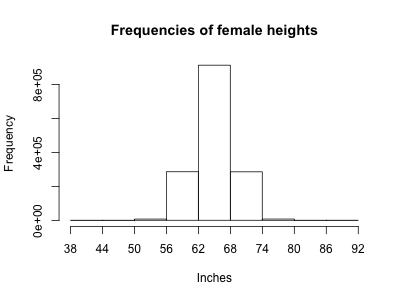
\includegraphics[scale=0.5]{figures/frequency-histogram-6.png}
%   %   \end{center}

% \end{frame}

% \begin{frame}
%   \frametitle{Height: histogram}

%   \begin{center}
%     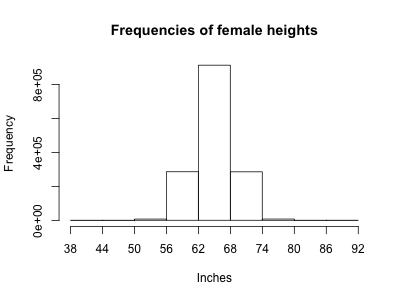
\includegraphics[scale=0.7]{figures/frequency-histogram-6.png}
%     \end{center}

% \end{frame}

% \begin{frame}
%   \frametitle{Height: barplot}

%   \begin{center}
%     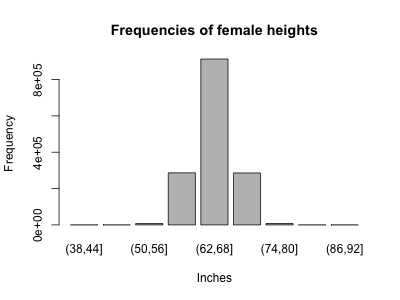
\includegraphics[scale=0.7]{figures/frequency-barplot-6.png}
%     \end{center}

% \end{frame}

% \begin{frame}
%   \frametitle{Height: h-plot}

%   \begin{center}
%     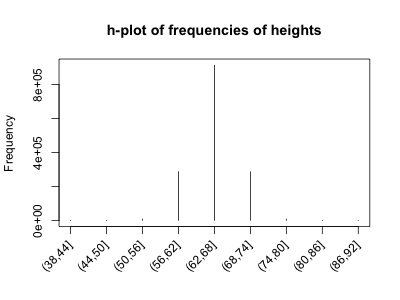
\includegraphics[scale=0.7]{figures/frequency-hplot-6.png}
%     \end{center}

% \end{frame}

% \begin{frame}
%   \frametitle{Height: relative frequency histogram}

%   \begin{center}
%     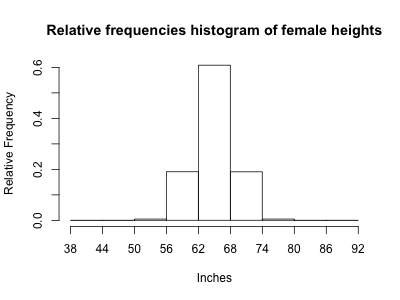
\includegraphics[scale=0.7]{figures/relfreq-histogram-6.png}
%     \end{center}

% \end{frame}

% \begin{frame}
%   \frametitle{Height: barplot (relative frequencies)}

%   \begin{center}
%     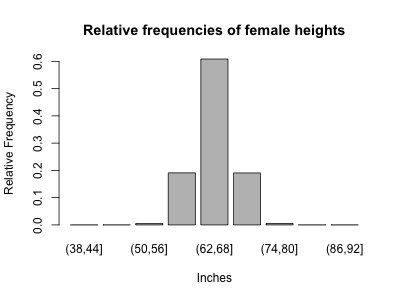
\includegraphics[scale=0.7]{figures/relfreq-barplot-6.png}
%     \end{center}

% \end{frame}

% \begin{frame}
%   \frametitle{Height: h-plot (relative frequencies)}

%   \begin{center}
%     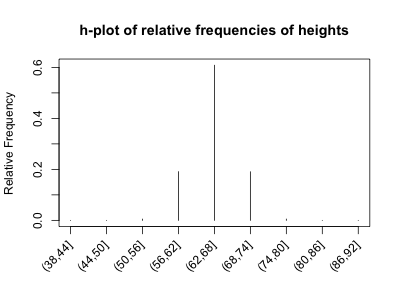
\includegraphics[scale=0.7]{figures/relfreq-hplot-6.png}
%     \end{center}

% \end{frame}

% \begin{frame}
%   \frametitle{Height: relative frequency histogram}

%   \begin{center}
%     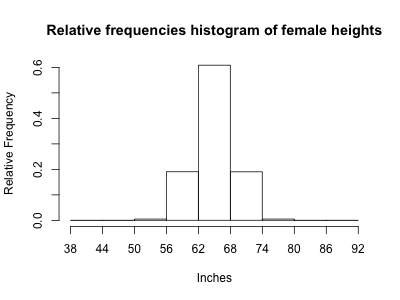
\includegraphics[scale=0.7]{figures/relfreq-histogram-6.png}
%     \end{center}

% \end{frame}

% \begin{frame}
%   \frametitle{Height: density histogram}

%   \begin{center}
%     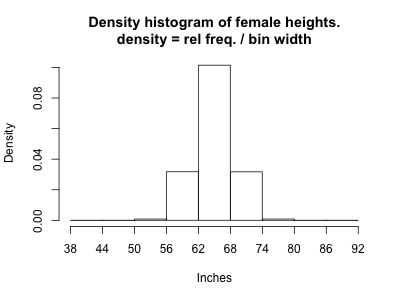
\includegraphics[scale=0.7]{figures/density-histogram-6.png}
%     \end{center}

%     $P(62 < \textmd{Height} \leq 68) = \textmd{area under curve between 56 and 62}$.

% \end{frame}

% \begin{frame}
%   \frametitle{Height: density histogram}

%   \begin{center}
%     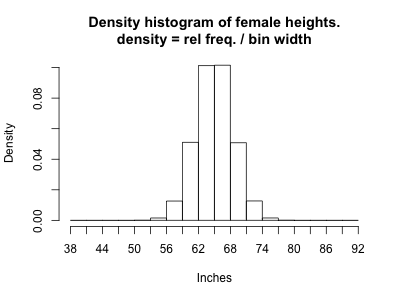
\includegraphics[scale=0.7]{figures/density-histogram-3.png}
%     \end{center}

% \end{frame}

% \begin{frame}
%   \frametitle{Height: density histogram}

%   \begin{center}
%     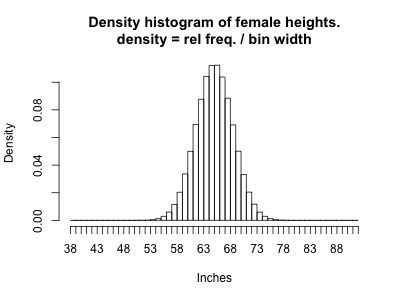
\includegraphics[scale=0.7]{figures/density-histogram-1.png}
%     \end{center}

% \end{frame}

% \begin{frame}
%   \frametitle{Height: density histogram}

%   \begin{center}
%     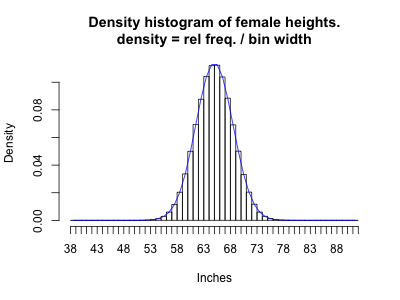
\includegraphics[scale=0.7]{figures/density-histogram-1-line.png}
%     \end{center}

% \end{frame}

% \begin{frame}
%   \frametitle{Height: probability density function}

%   \begin{center}
%     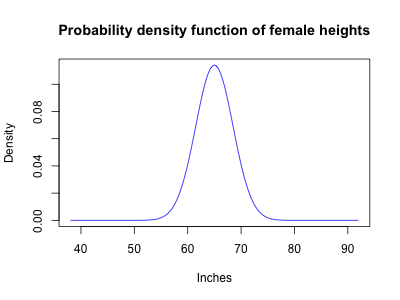
\includegraphics[scale=0.7]{figures/pdf-line.png}
%     \end{center}

% \end{frame}

%%%%%%%%%%%%%%%%%%%%%%%%%%%%%%%%%%%

\subsection{Normal distribution is unimodal, symmetric, and follows the 69-95-99.7 rule}
\label{mi2}

%%%%%%%%%%%%%%%%%%%%%%%%%%%%%%%%%%%%

\begin{frame}
\frametitle{2. Normal distribution is unimodal, symmetric, and follows the 69-95-99.7 rule}

\[ \mathhl{N(\mu,\sigma)} \]

\pause

\begin{itemize}

\item Unimodal and symmetric (bell shaped) that follows very strict guidelines about how variably the data are distributed around the mean \\

\pause

\item \hl{68-95-99.7 Rule:}
\begin{itemize}
\item about 68\% of the distribution falls within 1 SD of the mean
\item about 95\% falls within 2 SD of the mean
\item about 99.7\% falls within 3 SD of the mean
\item it is possible for observations to fall 4, 5, or more standard deviations away from the mean, but this is very rare if the data are nearly normal
\end{itemize}

\pause

\item While most variables are nearly normal, but none are exactly normal
% ALT ALT
% \item Lots of variables are nearly normal, but few are actually normal.

\end{itemize}

%---Note---%
\note{

Is it possible to make observations there are more than 3 sd from mean?

}

\end{frame}

%%%%%%%%%%%%%%%%%%%%%%%%%%%%%%%%%%%

\begin{frame}
\frametitle{}

\clicker{Speeds of cars on a highway are normally distributed with mean 65 miles / hour. The minimum speed recorded is 48 miles / hour and the maximum speed recorded is 83 miles / hour. Which of the following is most likely to be the standard deviation of the distribution?}

\begin{enumerate}[(a)]
\item -5 \only<2>{\soln{\darkgray{$\rightarrow$ SD cannot be negative}}}
\item \solnMult{5} \only<2>{\soln{\red{$\rightarrow 65 \pm (3 \times 5) = (50, 80)$}}}
\item 10 \only<2>{\soln{\darkgray{$\rightarrow 65 \pm (3 \times 10) = (35, 95)$}}}
\item 15 \only<2>{\soln{\darkgray{$\rightarrow 65 \pm (3 \times 15) = (20, 110)$}}}
\item 30 \only<2>{\soln{\darkgray{$\rightarrow 65 \pm (3 \times 30) = (-25, 155)$}}}
\end{enumerate}

%---Note---%
\note{

  Mine has them talk it over, even though plurality supports correct answer.
  Gives them a minute to talk about it.

  Asks someone to reason through answer.

}

\end{frame}

%%%%%%%%%%%%%%%%%%%%%%%%%%%%%%%%%%%

\subsection{Z scores serve as a ruler for any distribution}
\label{mi3}

%%%%%%%%%%%%%%%%%%%%%%%%%%%%%%%%%%%%

\begin{frame}
\frametitle{3. Z scores serve as a ruler for any distribution}

\disc{Would it be unusual for an adult woman in North Carolina to be 96'' (8 ft) tall?}

\pause

\hfill \\

\disc{Would it be unusual for an adult alien woman(?) to be 103 metreloots tall, assuming the distribution of heights is approximately normally distributed?}

\pause

\hfill \\

A Z score creates a common scale so you can assess data without worrying about the specific units in which it was measured.

\end{frame}

%%%%%%%%%%%%%%%%%%%%%%%%%%%%%%%%%%%

\begin{frame}
\frametitle{3. Z scores serve as a ruler for any distribution}

\[ Z = \frac{obs - mean}{SD} \]

\begin{itemize}

\item Z score: number of standard deviations it falls above or below the mean

\pause

\item Defined for distributions of any shape, but only when the distribution is normal can we use Z scores to calculate percentiles

\pause

\item Observations with $|Z| > 2$ are usually considered \hl{unusual}.

\end{itemize}

%---Note---%
\note{

Z: standardiZe.

Z score tells us number of standard deviations above or below the mean.

Defined for any distribution... this formula can be used for any distribution.
But if you are going to use them to calculate probabilities then you need a
normal distribution.

Convention says that observations that are more than 2 standard deviations away
are ``unusual.''

}

\end{frame}

%%%%%%%%%%%%%%%%%%%%%%%%%%%%%%%%%%%

\subsection{Z distribution is normal with $\mu = 0$ and $\sigma = 1$}
\label{mi4}

%%%%%%%%%%%%%%%%%%%%%%%%%%%%%%%%%%%%

\begin{frame}
\frametitle{4. Z distribution is normal with $\mu = 0$ and $\sigma = 1$}

\begin{itemize}

\item Linear transformations of a normally distributed random variable will also be normally distributed.

If
\[
X \sim N(\mu, \sigma)
\]
and
\[
Y = a + b \cdot X,
\]
then
\[
Y \sim N(a + b \cdot \mu, b \cdot \sigma).
\]

\end{itemize}

\end{frame}

%%%%%%%%%%%%%%%%%%%%%%%%%%%%%%%%%%%

\begin{frame}
\frametitle{4. Z distribution is normal with $\mu = 0$ and $\sigma = 1$}

\begin{itemize}

\item Hence, if

\[ Z = \frac{X - \mu}{\sigma}, \text{ where } X \sim N(\mu, \sigma), \]

then

\[ Z \sim N(0,1) \]

\item Z distribution is a special case of the normal distribution where $\mu = 0$ and $\sigma = 1$ (unit normal distribution)

\item The Z distribution is also called the ``standard normal'' distribution.

\end{itemize}

%---Note---%
\note{

A ``Z distribution'' is also commonly called a ``Standard normal distribution''.  Standard because it has mean zero and variance 1.

Z-score and calculator zoom example.

Going through class room example.  Heights of you.  Now computed z-score of each
of you would have standard normal distribution.

Really it is about creating a standard unit of measure.

Can we give an example?

}

\end{frame}

%%%%%%%%%%%%%%%%%%%%%%%%%%%%%%%%%%%

\begin{frame}
\frametitle{}

\clicker{Scores on a standardized test are normally distributed with a mean of 100 and a standard deviation of 20. If these scores are converted to standard normal Z scores, which of the following statements will be correct?}

\begin{enumerate}[(a)]
\item The mean will equal 0, but the median cannot be determined.
\item The mean of the standardized Z-scores will equal 100.
\item The mean of the standardized Z-scores will equal 5.
\item \solnMult{Both the mean and median score will equal 0.}
\item A score of 70 is considered unusually low on this test.
\end{enumerate}

%---Note---%
\note{

Read through clicker question.

Probably will be disagreement.  Have groups talk about it.

Go over it.
- Z score for mean of any distribution is 0.

Q. How will mean and median compare for a symmetric distribution?
A. They will be the same.

Thus the Z-score should be the same.

Look at (e) briefly.  How do I compute something that is ``unusual''...


}

\end{frame}

%%%%%%%%%%%%%%%%%%%%%%%%%%%%%%%%%%%

\begin{frame}
\frametitle{}

\vfill

\app{2.3 Normal distribution}{$\:$\\ See the course website for instructions. \\$\:$}

\vfill

%---Note---%
\note{

Give 15 minutes.  (Added time)

Tell the student's to
- Ask questions early so you don't get stuck.

- Show how to use tables.

}

\end{frame}

%%%%%%%%%%%%%%%%%%%%%%%%%%%%%%%%%%%

\begin{frame}

\clicker{Which of the following is \underline{false}?}

\begin{enumerate}[(a)]
\item Z scores are helpful for determining how unusual a data point is compared to the rest of the data in the distribution.
\item Majority of Z scores in a right skewed distribution are negative.
\item \solnMult{In a normal distribution, Q1 and Q3 are more than one SD away from the mean.}
\item Regardless of the shape of the distribution (symmetric vs. skewed) the Z score of the mean is always 0.
\end{enumerate}

\end{frame}

%%%%%%%%%%%%%%%%%%%%%%%%%%%%%%%%%%%%

\subsection{Normally distributed data plot as a straight line on the normal probability plot}
\label{mi5}

%%%%%%%%%%%%%%%%%%%%%%%%%%%%%%%%%%%%

\begin{frame}
\frametitle{Anatomy of a normal probability plot}

\begin{itemize}

\item Data are plotted on the y-axis of a normal probability plot, and theoretical quantiles (following a normal distribution) on the x-axis

\pause

\item If there is a linear relationship between the data and the theoretical quantiles, then the data follow a nearly normal distribution

\pause

\item Since a linear relationship would appear as a straight line on a scatter plot, the closer the points are to a perfect straight line, the more confident we can be that the data follow the normal model

\pause

\item Constructing a normal probability plot requires calculating percentiles and corresponding Z-scores for each observation, which is tedious. Therefore we generally rely on software when making these plots

\end{itemize}

\end{frame}

%%%%%%%%%%%%%%%%%%%%%%%%%%%%%%%%%%%


\begin{frame}
\frametitle{Normal probability plot}

A histogram and \hl{normal probability plot} of a sample of 100 male heights.

\begin{center}
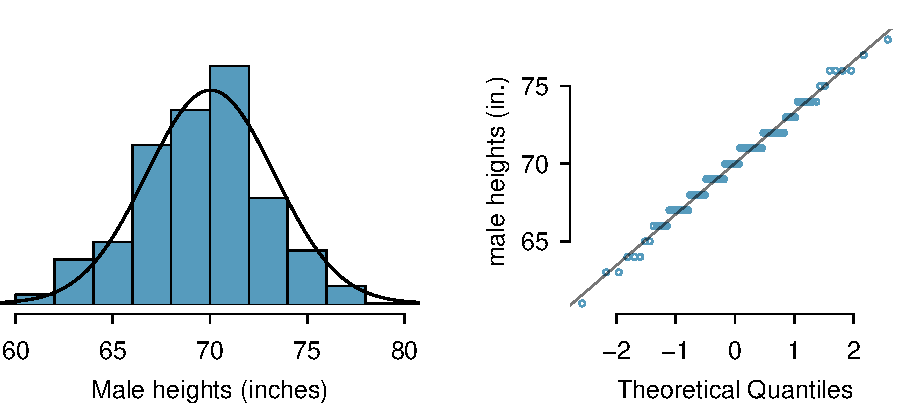
\includegraphics[width=0.9\textwidth]{figures/fcidMHeights/fcidMHeights}
\end{center}

\disc{Why do the points on the normal probability have jumps?}

\end{frame}

%%%%%%%%%%%%%%%%%%%%%%%%%%%%%%%%%%%

\begin{frame}
\frametitle{Constructing a normal probability plot}

We construct a normal probability plot for the heights of a sample of 100 men as follows:

\begin{enumerate}

\item Order the observations.

\item Determine the percentile of each observation in the ordered data set.

\item Identify the Z scores corresponding to the each percentile \emph{for a Z distribution}.

\item Create a scatterplot of the observations (vertical) against the Z scores (horizontal)

\end{enumerate}

\pause

\begin{center}
\begin{tabular}{l | c | c | c | c | c}
Observation $i$	& 1		& 2		& 3		& $\cdots$	& 100 \\
\hline
$x_i$			& 61		& 63		& 63		& $\cdots$	& 78 \\
Percentile	, $i / (n+1)$& 0.99\% 	& 1.98\% 	& 2.97\% 	& $\cdots$	& 99.01\% \\
$z_i$			& -2.33	& -2.06 	& -1.89	& $\cdots$	& 2.33
\end{tabular}
\end{center}

\pause

\disc{How are the Z scores corresponding to each percentile determined?}

\end{frame}

%%%%%%%%%%%%%%%%%%%%%%%%%%%%%%%%%%%

\begin{frame}

\disc{Below is a histogram and normal probability plot for the heights of Duke men's basketball players (from 1990s and 2000s). Do these data appear to follow a normal distribution?}

\begin{center}
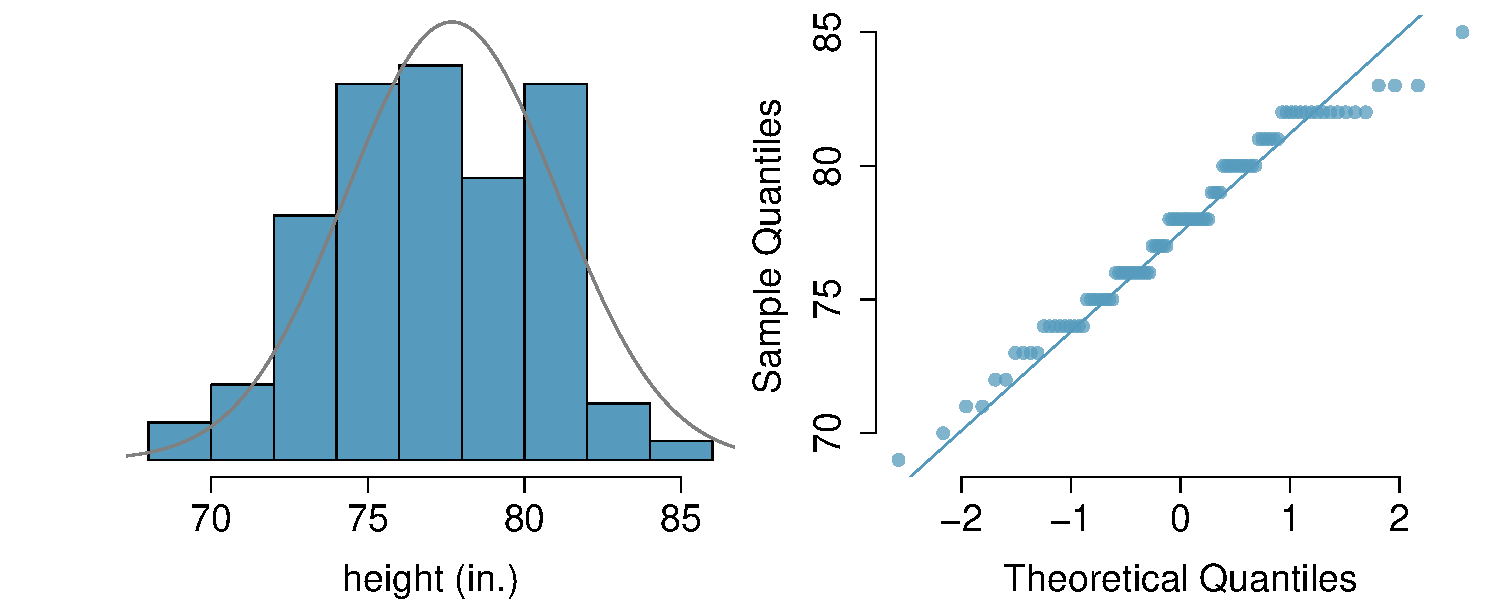
\includegraphics[width=\textwidth]{figures/qq_duke/qq_duke}
\end{center}

\vfill

\ct{Source: GoDuke.com}

\end{frame}

%%%%%%%%%%%%%%%%%%%%%%%%%%%%%%%%%%%

\begin{frame}
\frametitle{Normal probability plot and skewness}

\twocol{0.35}{0.65}{
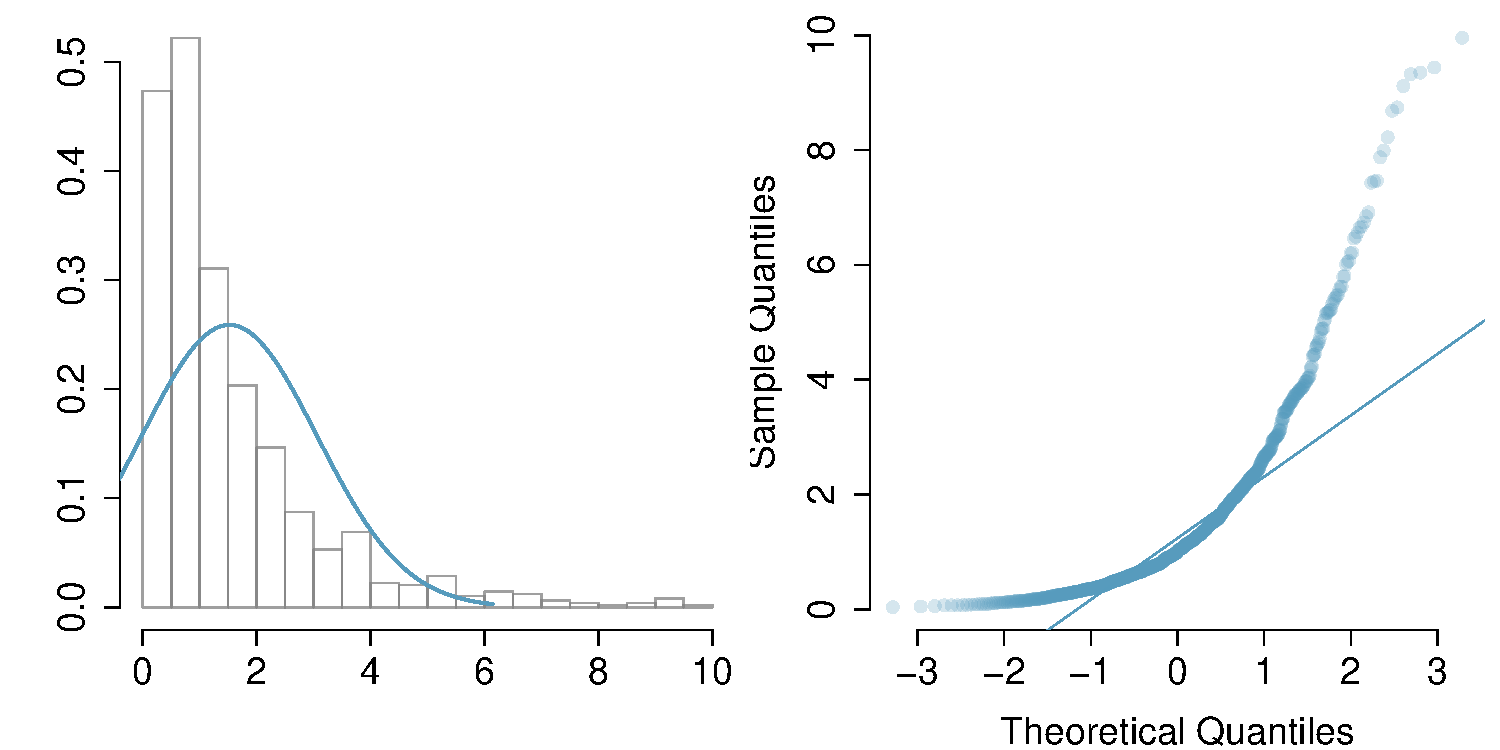
\includegraphics[width=\textwidth]{figures/qqnorm/right_skew} 
}
{
Right Skew - Points bend up and to the left
}

\pause
\twocol{0.35}{0.65}{
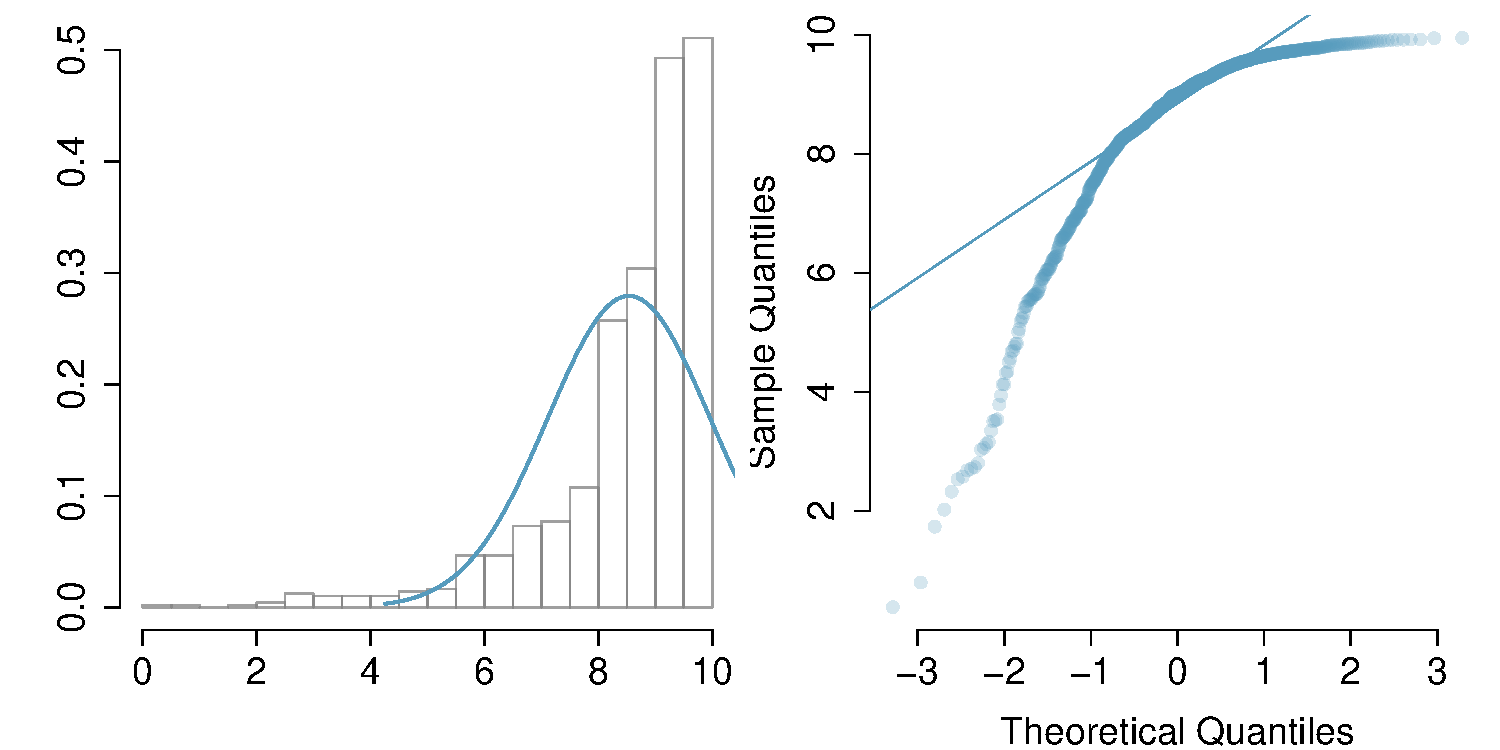
\includegraphics[width=\textwidth]{figures/qqnorm/left_skew} 
}
{
Left Skew - Points bend down and to the right 
}

\pause
\twocol{0.35}{0.65}{
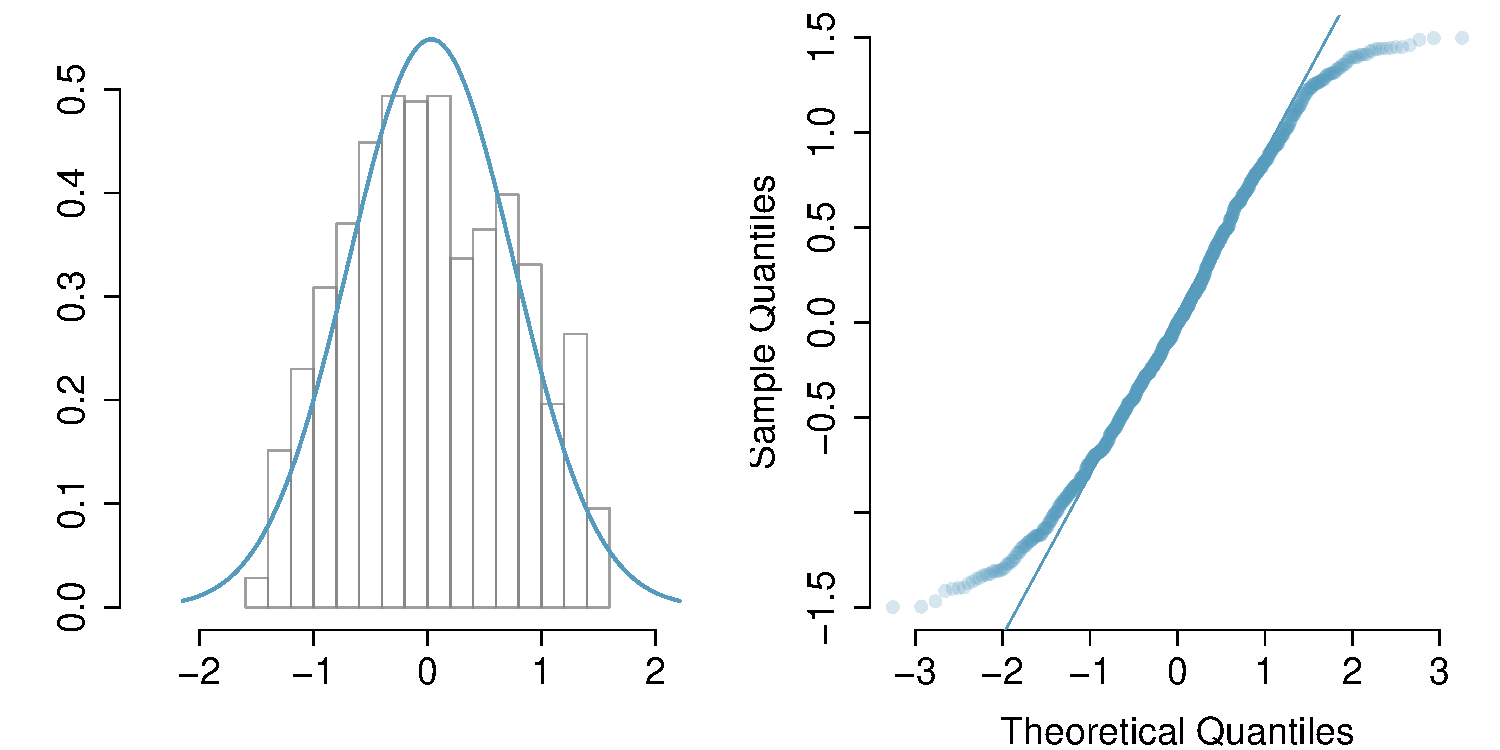
\includegraphics[width=\textwidth]{figures/qqnorm/skinny_tails} 
}
{
Skinny Tails - S shaped-curve indicating shorter than normal tails (narrower, less variable, than expected)
}

\pause
\twocol{0.35}{0.65}{
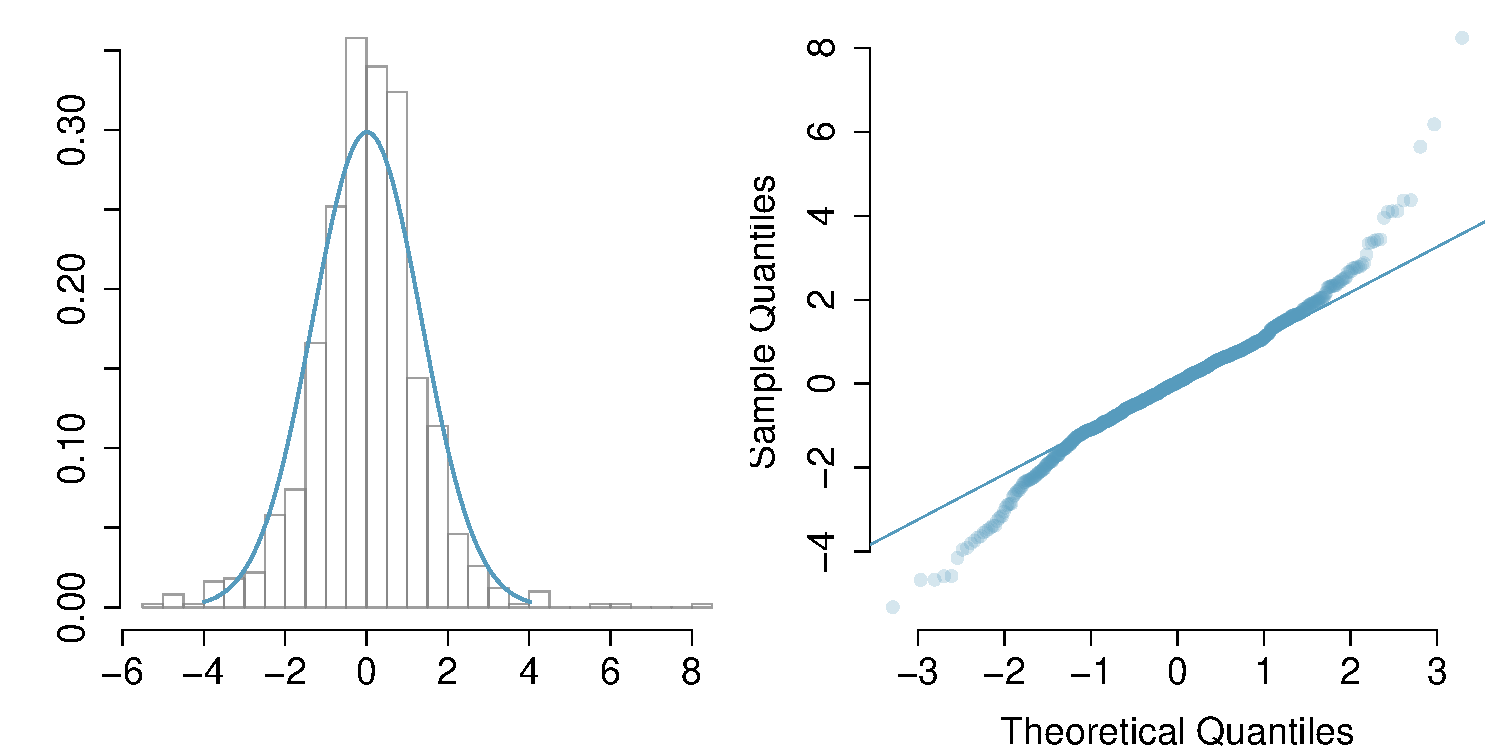
\includegraphics[width=\textwidth]{figures/qqnorm/fat_tails} 
}
{
Fat Tails - Curve starting below the normal line, bends to follow it, and ends above it (wider, more variable, than expected)
}

\end{frame}

%%%%%%%%%%%%%%%%%%%%%%%%%%%%%%%%%%%

\section{Summary}

%%%%%%%%%%%%%%%%%%%%%%%%%%%%%%%%%%%

\begin{frame}
\frametitle{Summary of main ideas}

\vfill

\begin{enumerate}

\item \nameref{mi1}

\item \nameref{mi2}

\item \nameref{mi3}

\item \nameref{mi4}

\item \nameref{mi5}

\end{enumerate}

\vfill

\end{frame}

%%%%%%%%%%%%%%%%%%%%%%%%%%%%%%%%%%%

\section{Exercise [time permitting]}

%%%%%%%%%%%%%%%%%%%%%%%%%%%%%%%%%%%

\begin{frame}
\frametitle{}

\disc{{\small At a pharmaceutical factory the amount of the active ingredient which is added to each
pill is supposed to be 36 mg. The amount of the active ingredient added follows a nearly
normal distribution with a standard deviation of 0.11 mg. Once every 30 minutes a pill
is selected from the production line, and its composition is measured precisely. We know that the failure rate of the quality control is 3\% at this factory. What are the bounds of the acceptable amount of the active ingredient?}}

\end{frame}

%%%%%%%%%%%%%%%%%%%%%%%%%%%%%%%%%%%

\end{document}